% Created 2022-12-10 Sat 11:43
% Intended LaTeX compiler: pdflatex
\documentclass[11pt]{article}
\usepackage[utf8]{inputenc}
\usepackage[T1]{fontenc}
\usepackage{graphicx}
\usepackage{longtable}
\usepackage{wrapfig}
\usepackage{rotating}
\usepackage[normalem]{ulem}
\usepackage{amsmath}
\usepackage{amssymb}
\usepackage{capt-of}
\usepackage{hyperref}
\author{Daniel Rosel}
\date{\today}
\title{Discrete Mathematics - Final}
\hypersetup{
 pdfauthor={Daniel Rosel},
 pdftitle={Discrete Mathematics - Final},
 pdfkeywords={},
 pdfsubject={},
 pdfcreator={Emacs 28.2 (Org mode 9.5.5)},
 pdflang={English}}
\begin{document}

\maketitle
\setcounter{tocdepth}{2}
\tableofcontents




\section{Domains}
\label{sec:org7b5b900}
\begin{description}
\item[{Naturals \(\mathbb{N}\)}] \([1,2,3,\ldots,\infty)\)
\item[{Integers \(\mathbb{Z}\)}] \((-\infty,\ldots,-2,0,2,\ldots,\infty)\)
\item[{Rationals \(\mathbb{Q}\)}] Fractions of integers \(\{ \frac{p}{q} \vert p \in Z \land q \in Z \land q \ne 0 \}\)
\item[{Reals \(\mathbb{R}\)}] All real numbers
\item[{Complex \$\mathbb{C}}] All complex numbers
\end{description}
\section{Terminology}
\label{sec:orgf584ba4}
\begin{description}
\item[{Theorem}] A statement we can prove using some axioms
\item[{Proof}] A valid argument/set of arguments that demonstrate a theorem/proposition
\item[{Axioms}] Statements which are assumed to be true, they are in the most basic form
\item[{Lemma}] A small proof that is an element of another larger proof
\end{description}
\section{Propositional Logic}
\label{sec:org2971812}
A proposition, is a sentence, which can be given some \textbf{truth value}.
There are two types of propositions:
\begin{description}
\item[{Tautology}] A proposition that will always be \textbf{true} (\(\top\))
\item[{Contradiction}] A proposition that will never be true (\(\bot\))
\end{description}
\subsection{Operators}
\label{sec:org3154298}
There are three main operators which can be used to express any logical expression. These consists of \textbf{Not, Conjunction, Disjunction}.
\subsubsection{Not}
\label{sec:orgf190e6a}
It flips the truth value of a proposition.

\[
\neg p, \bar{A}
\]
\subsubsection{Conjunction}
\label{sec:org7864529}
This operators returns a new truth value which is true \textbf{if both of the propositions are true}

\[
p \land q, AB
\]
\subsubsection{Disjunction}
\label{sec:orgcac3798}
Like the conjunction, it operates on two propositions. It will return true as long as either of the propositions is true.

\[
p \lor q, A+B
\]
\subsubsection{Exclusive OR (XOR)}
\label{sec:org4fd5d08}
It is very similar to the \textbf{Disjunction} except that it must be exclusively one value that is true.

\[
p \oplus q = (p \lor q) \land \neg(p \land q)
\]

\subsubsection{Conditional Statements / Implication}
\label{sec:org7870440}
A conditional statement consists of two parts, the \textbf{premise} and \textbf{consequence}. The truth value is \textbf{only false when \(T \to F\)}.

\[
p \to q \equiv \neg p \lor q
\]

\begin{itemize}
\item If \(p\) is True, then \(q\) must also be True, we say that p is a \textbf{sufficient condition} for \(q\). \(T \to T\)
\item If \(p\) is False, \(q\) could still be True. \(F \to T\)
\item \(p\) cannot be true if \(q\) is not true. \(F \to F\)
\item \(p\) could still be false, even if \(q\) is true. \(F \to T\)
\end{itemize}

\[
((p \to q) \land p) \to q
\]

\[
((p \to q) \land \neg q) \to \neg p
\]

\subsubsection{Bi-conditionals}
\label{sec:orgff9ef26}
It expressed a \textbf{sufficient} and \textbf{necessary} conditional relationship between two propositions. It is read as \emph{if and only if p, then q}.

\[
p \Leftrightarrow q
\]

This operator will return True only if both p and q have equal values. The expression can be represented with the 3 basic operators as:

\[
(p \to q) \land (q \to p) \equiv (\neg p \land \neg q) \lor (p \land q)
\]

\[
p \equiv q = \neg (p \oplus q)
\]

\subsubsection{Order of Operators}
\label{sec:orgd68dfd2}
\begin{enumerate}
\item \(\neg\)
\item \(\land\)
\item \(\lor\)
\item \(\to\)
\item \(\Leftrightarrow\)
\end{enumerate}

\subsection{DeMorgan's Laws}
\label{sec:org55a97fc}
\begin{align}
\neg (p \land q) \equiv \neg p \lor \neg q \\
\neg (p \lor q) \equiv \neg p \land q
\end{align}

\subsection{Fallacies}
\label{sec:org7c58c46}
The fallacies stem from the fact that an implication is true, and the truth value of either \(p,q\).
\begin{description}
\item[{Affirming the consequent}] \(((p \to q) \land q) \to p\). We falsely assume that the premise is \textbf{true} because the consequence is \textbf{true}
\item[{Nageting the antecedent}] \(((p \to q) \land \neg p) \to \neg q\). We falsely assume that the consequence is \textbf{false} because the premise is \textbf{false}.
\end{description}

\subsection{Converse, Contrapositive, Inverse}
\label{sec:org3739445}
\begin{description}
\item[{Converse}] \(q \to p\)
\item[{Contrapositive}] \(\neg q \to \neg p\)
\item[{Inverse}] \(\neg p \to \neg q\)
\end{description}

The fallacies are a product of assuming that the \textbf{Converse and Inverse} are equivalent to the conditional statement.
\subsection{Disjunctive Normal Form}
\label{sec:org5490d3f}
This is a proposition created from the values in the truth table.

\subsection{Logical Equivalences}
\label{sec:org8067ec4}
These are various way you can arrive at some conclusion given a few basic propositions.
\subsubsection{Identity Laws}
\label{sec:org714fea5}
\[
p \land \top \equiv p
\]

\[
p \lor \bot \equiv p
\]
\subsubsection{Denomination Laws}
\label{sec:orgaf01463}
\[
p \lor \top \equiv \top
\]

\[
p \land \bot \equiv \bot
\]
\subsubsection{Idempotent Laws}
\label{sec:org9f01ea5}
\[
p \lor p \equiv p
\]

\[
p \land p \equiv p
\]
\subsubsection{Double Negation Law}
\label{sec:org80e86fc}
\[
\neg ( \neg p) \equiv p
\]
\subsubsection{Commutative Laws}
\label{sec:org84ea1dd}
\[
p \lor q \equiv q \lor p
\]

\[
p \land q \equiv q \land p
\]
\subsubsection{Associative Laws}
\label{sec:org1514741}
\[
(p \lor q) \lor r \equiv p \lor (q \lor r)
\]

\[
(p \land q) \land r \equiv p \land (q \land r)
\]
\subsubsection{Distributive Laws}
\label{sec:org29c8fe4}
\[
p \lor (q \land r) \equiv (p \lor q) \land (p \lor r)
\]

\[
p \land (q \lor r) \equiv (p \land q) \lor (p \land r)
\]
\subsubsection{\ref{sec:org55a97fc}}
\label{sec:org4cadf10}
\subsubsection{Absorption Laws}
\label{sec:orgaf8e2c4}
\[
p \lor (p \land q) \equiv p
\]

\[
p \land (p \lor q) \equiv p
\]
\subsubsection{Negation Laws}
\label{sec:org54b5b71}
\[
p \lor \neg p \equiv \top
\]

\[
p \land \neg p \equiv \bot
\]
\subsection{Satisfiability}
\label{sec:org1973582}
A proposition is satisfiable if it has at least one case for which it is \textbf{true}, it is anything but a \textbf{contradiction}.
\subsection{Practice Problems}
\label{sec:orgab97247}
For the following, create a truth table and a DNF for each (a DNF is a proposition created from the values in the truth table)
\begin{enumerate}
\item \(p \lor \neg p\)

Truth Table:

\begin{array}{|c|c|c|}
\hline
p & \neg p & p \lor \neg p \\
\hline
T & F & T \\
\hline
F & T & T \\
\hline
\end{array}

DNF:

\[
    p \lor \neg p = \top
    \]

\item \(p \land \neg p\)

Truth Table:

\begin{array}{|c|c|c|}
\hline
p & \neg p & p \land \neg p \\
\hline
T & F & F \\
\hline
F & T & F \\
\hline
\end{array}

DNF:

\[
    p \land \neg p = \bot
    \]
\item \(p \lor (p \land q)\)

Truth Table:

\begin{array}{|c|c|c|}
\hline
p & q & p \lor (p \land q) \\
\hline
T & T & T \\
\hline
T & F & T \\
\hline
F & T & F \\
\hline
F & F & F \\
\hline
\end{array}

DNF:

\[
    p \lor (p \land q) = p
    \]
\item \(p \land (p \lor q)\)

Truth Table:
\begin{array}{|c|c|c|}
\hline
p & q & p \land (p \lor q) \\
\hline
T & T & T \\
\hline
T & F & T \\
\hline
F & T & F \\
\hline
F & F & F \\
\hline
\end{array}

DNF:

\[
    p \land (p \lor q) = p
    \]
\end{enumerate}

Now for implications:
\begin{enumerate}
\item \(p \to q\)

Truth Table:

\begin{array}{|c|c|c|}
\hline
p & q & p \to q \\
\hline
T & T & T \\
\hline
T & F & F \\
\hline
F & T & T \\
\hline
F & F & T \\
\hline
\end{array}

DNF:

\[
    p \to q = \neg p \lor q
    \]
\item \(p \to \neg q\)

Truth Table:

\begin{array}{|c|c|c|}
\hline
p & q & p \to \neg q \\
\hline
T & T & F \\
\hline
T & F & T \\
\hline
F & T & T \\
\hline
F & F & T \\
\hline
\end{array}

DNF:

\[
    p \to \neg q = \neg p \lor \neg q
    \]
\item \((\neg p) \to q\)

Truth Table:

\begin{array}{|c|c|c|}
\hline
p & q & (\neg p) \to q \\
\hline
T & T & T \\
\hline
T & F & T \\
\hline
F & T & T \\
\hline
F & F & F \\
\hline
\end{array}

DNF:

\[
    (\neg p) \to q = p \lor q
    \]
\item \(\neg p \to \neg q\)

Truth Table:

\begin{array}{|c|c|c|}
\hline
p & q & \neg p \to \neg q \\
\hline
T & T & T \\
\hline
T & F & T \\
\hline
F & T & F \\
\hline
F & F & T \\
\hline
\end{array}

DNF:

\[
    \neg p \to \neg q = p \lor \neg q
    \]
\end{enumerate}

Prove the following:
\begin{enumerate}
\item \(p \to q \equiv \neg p \lor q\)

Proof:

\begin{array}{|c|c|c|}
\hline
p & q & p \to q & \neg p \lor q \\
\hline
T & T & T & T \\
\hline
T & F & F & F \\
\hline
F & T & T & T \\
\hline
F & F & T & T \\
\hline
\end{array}

Therefore \(p \to q \equiv \neg p \lor q\) is true.

\item \(p \to q \equiv \neg q \to \neg p\)

Proof:

\begin{array}{|c|c|c|}
\hline
p & q & p \to q & \neg q \to \neg p \\
\hline
T & T & T & T \\
\hline
T & F & F & F \\
\hline
F & T & T & T \\
\hline
F & F & T & T \\
\hline
\end{array}

Therefore \(p \to q \equiv \neg q \to \neg p\) is true.
\end{enumerate}

Which of the following are satisfiable:
\begin{enumerate}
\item \(p \land \neg p\)

\begin{array}{|c|c|c|}
\hline
p & \neg p & p \land \neg p \\
\hline
T & F & F \\
\hline
F & T & F \\
\hline
\end{array}

Therefore \(p \land \neg p\) is unsatisfiable.
\item \(p \lor \neg p\)

\begin{array}{|c|c|c|}
\hline
p & \neg p & p \lor \neg p \\
\hline
T & F & T \\
\hline
F & T & T \\
\hline
\end{array}

Therefore \(p \lor \neg p\) is satisfiable.
\item \(p \to q\)

\begin{array}{|c|c|c|}
\hline
p & q & p \to q \\
\hline
T & T & T \\
\hline
T & F & F \\
\hline
F & T & T \\
\hline
F & F & T \\
\hline
\end{array}

Therefore \(p \to q\) is satisfiable.
\item \(p \to \neg q\)

\begin{array}{|c|c|c|}
\hline
p & q & p \to \neg q \\
\hline
T & T & F \\
\hline
T & F & T \\
\hline
F & T & T \\
\hline
F & F & T \\
\hline
\end{array}

Therefore \(p \to \neg q\) is satisfiable.
\item \(\neg p \to q\)

\begin{array}{|c|c|c|}
\hline
p & q & \neg p \to q \\
\hline
T & T & T \\
\hline
T & F & T \\
\hline
F & T & T \\
\hline
F & F & F \\
\hline
\end{array}

Therefore \(\neg p \to q\) is satisfiable.
\end{enumerate}

\section{Predicate Logic}
\label{sec:orgc6379fa}
With predicate logic, we can break down a complex proposition into predicates and quantifiers.

\subsection{Predicates}
\label{sec:orgac11690}
It is a statement, which is made up of a proposition, with the only difference being that it can take a parameter.

\begin{array}{l}
X \text{ is faster than me} \\
= \text{Subject} + \text{Predicate} \\
\to P(x)
\end{array}

We say that the it is instantiated once it gets evaluated with the passed parameter.

\[
P(x_1, x_2, x_3, \ldots, x_n)
\]

And once instantiated with variables:

\[
P(a_1, a_2, a_3, \ldots, a_n) \equiv p
\]

\subsection{Quantifiers}
\label{sec:org5f099a8}
With a quantifier, we can specify for which values on a certain domain, a predicate is true of false. There are various ways to express this: (\textbf{for all}, \textbf{for many}, \textbf{for at least one}, \textbf{for none}).

\subsection{Universal Quantifier}
\label{sec:org689ca38}
If we have some predicate for which we can say that all the possible values in a certain domain will make it true, we use the universal quantifier.

\begin{array}{c}
P(x) \text{ for all value of x within its domain} \\
\forall x P(x)
\end{array}

\begin{itemize}
\item To prove that this quantifier is true, we must demonstrate that it holds true for all the possible values.
\item To \textbf{dis}-prove the quantifier, it is sufficient to show that there exists just one that does not satisfy the predicate
\item If we are considering an empty set, it will always be false.
\end{itemize}

\subsection{Existential Quantifier}
\label{sec:org03a6e55}
\begin{array}{c}
P(x) \text{ for at least one value of x within its domain} \\
\exists x P(x)
\end{array}

\begin{itemize}
\item To prove this quantifier, we must find at least one value for which the predicate holds true
\item To disprove the quantifier, we must show that all the values will not hold for the predicate
\item Again, if we consider and empty set, it will always be false
\end{itemize}

\subsection{Singular Existential Quantifier}
\label{sec:org5dd2276}
We can also use the existential quantifier, and with a bit of modification we can use it to specify how many values will satisfy the predict.

\begin{array}{c}
\text{There is exactly one } x \text{ such that } P(x) \\
\exists! x P(x)
\end{array}

The definition for this is as follows:

\[
\exists x (P(x) \land \forall y (P(y) \Leftrightarrow x = y))
\]

We can generalize this to a specific number \(n\) for which the predicate is satisfiable.

\[
\exists_n x P(x)
\]

\subsection{Negation}
\label{sec:org1f16761}
When negating a quantifier, we have to consider both the outside and inside, that being \textbf{the quantifier itself} and the \textbf{predicate}.

\[
\neg \forall x P(x) \equiv \exists x \neg P(x)
\]

\[
\neg \exists x P(x) \equiv \forall x \neg P(x)
\]

\subsection{Nesting}
\label{sec:org01dface}
If we have more than one variable for which we quantify a predicate, we have to \textbf{consider the order}.

\[
\exists x \forall y P(x,y) \not \equiv \forall y \exists x P(x,y)
\]

\subsection{Practice Problems}
\label{sec:orgd3e4854}
Evaluate the following:
\begin{enumerate}
\item \(\forall x \exists y P(x,y)\) where \(P(x,y) = x > y\)

This quantifier is true, because for any value of \(x\), there will always be a value of \(y\) that will satisfy the predicate.
\item \(\exists x \forall y P(x,y)\) where \(P(x,y) = x > y\)

This quantifier is false, because there will always be a value of \(x\) for which there will not be a value of \(y\) that will satisfy the predicate.
\item \(\forall x \exists y P(x,y)\) where \(P(x,y) = x < y\)

This quantifier is true, because for any value of \(x\), there will always be a value of \(y\) that will satisfy the predicate. This because no matter the value of \(x\), there will always be a value of \(y\) that will be greater than \(x\).
\end{enumerate}

Prove the following:
\begin{enumerate}
\item \(\forall x \exists y P(x,y) \equiv \exists y \forall x P(x,y)\)
\end{enumerate}

Nested quantifiers:
\begin{enumerate}
\item \(\exists x \forall y \exists z P(x,y,z)\) where \(P(x,y,z) = x > y \land y > z\)
\end{enumerate}

Negating quantifiers:
\begin{enumerate}
\item \(\neg \forall x \exists y P(x,y)\) where \(P(x,y) = x > y\)
\end{enumerate}

\section{Inference}
\label{sec:org3687601}
A process of arriving at some conclusion through logical steps. This process consists of \textbf{arguments} which can either be valid or not. The logical form of an argument is vital, because it is the only way to determine if it is true or not.

\begin{array}{r}
p \to q \\ p
\\
\hline
\therefore q
\end{array}


It is another thing to call an argument \textbf{sound}, for this we need to have an argument for which \textbf{all premises are true and valid}. \textbf{A valid argument implies a tautology}. How can we tell if an argument is valid? We can use the \textbf{truth table}. Another way to determine if an argument is valid is to see if it makes use of any \textbf{existing argument forms}.

\subsection{Rules of Inference}
\label{sec:org77e60f1}
An argument form which would generate a valid implication falls under the rules of inference
\subsubsection{Modus Ponens}
\label{sec:org7b8e6d4}

\begin{array}{r}
p \\
p \to q
\\
\hline
q
\end{array}


\begin{enumerate}
\item If p is true, then q is true
\item p is true
\item Therefore q is true
\end{enumerate}
\subsubsection{Modus Tollens}
\label{sec:org3a78aa0}


\begin{array}{r}
\neg q \\
p \to q
\\
\hline
\neg p
\end{array}

\subsubsection{Hypothetical Syllogism}
\label{sec:org1c8a2f6}

\begin{array}{r}
p \to q \\
q \to r
\\
\hline
p \to r
\end{array}

\subsubsection{Disjunctive Syllogism}
\label{sec:orgdf3788a}

\begin{array}{r}
p \lor q \\
\neg p
\\
\hline
q
\end{array}

\subsubsection{Addition}
\label{sec:orgfb64f32}

\begin{array}{r}
p
\\
\hline
p \lor q
\end{array}

\subsubsection{Simplification}
\label{sec:org284a162}

\begin{array}{r}
p \land q
\\
\hline
p
\end{array}

\subsubsection{Conjunction}
\label{sec:org38f4167}

\begin{array}{r}
p \\ q
\\
\hline
p \land q
\end{array}

\subsubsection{Resolution}
\label{sec:org1600aad}

\begin{array}{r}
p \lor q \\
\neg p \lor r
\\
\hline
\therefore q \lor r
\end{array}

\subsection{Rules of Inference for Quantified Propositions}
\label{sec:orgc465c0d}
\subsubsection{Universal Instantiation}
\label{sec:org2074e16}
\begin{array}{r}
\forall x P(x)
\\
\hline
\therefore P(c)
\end{array}

\subsubsection{Universal Generalization}
\label{sec:org324f934}
\begin{array}{r}
P(c) \text{ for an arbitrary c}
\\
\hline
\therefore \forall x P(x)
\end{array}

\subsubsection{Existential Instantiation}
\label{sec:org02d9b51}
\begin{array}{r}
\exists x P(x)
\\
\hline
\therefore P(c)
\end{array}

\subsubsection{Existential Generalization}
\label{sec:org15609e9}
\begin{array}{r}
P(c) \text{ for an arbitrary c} \\
\hline
\therefore \exists x P(x)
\end{array}

\subsection{Practice Problems}
\label{sec:org784b60f}
Use the rules of inference to prove the following:
\begin{enumerate}
\item \(\neg (p \lor q) \to \neg p \land \neg q\)

\begin{array}{r}
\neg (p \lor q) \\
p \lor q
\\
\hline
\therefore \neg p \land \neg q
\end{array}

The rules of inference used are Modus Tollens and Disjunctive Syllogism.
\item \(\neg (p \land q) \to \neg p \lor \neg q\)

\begin{array}{r}
\neg (p \land q) \\
p \land q
\\
\hline
\therefore \neg p \lor \neg q
\end{array}

The rules of inference used are Modus Tollens and Conjunction.
\end{enumerate}

Prove the following using the rules of inference for quantified propositions:
\begin{enumerate}
\item \(\forall x P(x) \to P(c)\) where \(P(x) = x > 0\)

\begin{array}{r}
\forall x P(x) \\
P(c)
\\
\hline
\therefore P(c)
\end{array}

The rules of inference used are Universal Instantiation.

\item \(\exists x P(x) \to P(c)\) where \(P(x) = x > 0\)

\begin{array}{r}
\exists x P(x) \\
P(c)
\\
\hline
\therefore P(c)
\end{array}

The rules of inference used are Existential Instantiation.
\end{enumerate}

Turn the following phrases into logical statements using the rules of inference for quantified propositions:
\begin{enumerate}
\item For all \(x\), \(x > 0\)

\(\forall x (x > 0)\)
\item There exists \(x\) such that \(x > 0\)

\(\exists x (x > 0)\)
\item There exists \(x\) such that \(x > 0\) and \(x < 10\)

\(\exists x (x > 0 \land x < 10)\)
\end{enumerate}

\section{Formal Proofs}
\label{sec:org570b4e6}
This kind of proof is made up of statements which we can infer from previous statements. This we can construct using a table in which we state the logical expression and how we got to it.

\begin{align}
(p \lor q) \to (r \land s) & \quad \text{Premise} \\
r \to t & \quad \text{Premise} \\
\neg t & \quad \text{Premise} \\
\neg r & \quad \text{Modus Tollens from 2 and 3} \\
(\neg p \land \neg q) & \quad \text{Modus Tollens from 4 and 1} \\
\neg p & \quad \text{Simplification of 5}
\end{align}

\section{Informal Proofs}
\label{sec:orgf3b7432}
Because a formal proof can get convoluted, we use informal proofs. The main difference here is that we don't need to provide a step-by-step description of how the proof works; we just show how the conclusion is true by describing a few intermediate steps between the theorem and the corollary. (These are called \textbf{premises} and \textbf{conclusions} in logic.)
There are various methods of proof we can use. The two primary categories for these proofs are \textbf{direct} and \textbf{indirect}.

\subsection{Methods of Proof}
\label{sec:org05f992f}
Upon deciding which axioms to use, you then need to use some method of proof. The most common statements we will be proving are implications.
\subsubsection{Direct Proof}
\label{sec:org4d5c5ad}
We want to prove \textbf{"If p, then q}". This is done by assuming that the \textbf{premise} is true and then proving that the consequence is also true.

\begin{enumerate}
\item We assume \(p\) to be true.
\item By applying the laws of inference, we deduce \(q\) from \(p\).
\end{enumerate}
\subsubsection{Indirect: Proof by Contraposition}
\label{sec:org4a2fe31}
If we cannot arrive to the consequence using just the premise, we can use contraposition, which states that \((p \to q) \equiv (\neg q \to \neg p)\).

\begin{enumerate}
\item We assume that \(\neg q\) is true
\item We find a way to infer that \(\neg p\) is true
\item Since this verifies the contrapositive, we have proved that \(p \to q\)
\end{enumerate}

\subsubsection{Indirect: Vacuous and Trivial proofs}
\label{sec:orgf8b3699}
If we are saying that \(p \to q\) is \textbf{True}, we can assume that:
\begin{enumerate}
\item \(p\) is False (Vacuous proof)
\item \(q\) is True (Trivial proof)
\end{enumerate}

It is enough to prove just one of these (as long as we do not accept the premise being True) we can prove the condition to be True.
\begin{enumerate}
\item Example
\label{sec:org2d59bdd}
If \(n\) is an integer and an even number, then \(2n\) must be an integer.
\begin{description}
\item[{Solution}] Since an integer multiplied by another integer will also be an integer, we can say that \(q\) will be true. This is enough to prove that \(p \to q\) is also True.
\end{description}
\end{enumerate}
\subsubsection{Indirect: Proof by Contradiction}
\label{sec:org1a78359}
This can be used to demonstrate any statement \(p\). We say that \(\neg p\) implies a contradiction. A nicer way to think about this is by the following:

\[
\neg p \to \bot \equiv \neg (\neg p) \lor \bot \equiv p \lor \bot \equiv p
\]

If we should use proof by contradiction on an implication, we must prove that \(p \land \neg q \to \bot\). This is because in this case, we need to show that the negation of the implication is a contradiction.

\[
\neg (p \to q) \equiv \neg (\neg p \lor q) \equiv p \land \neg q \equiv \bot
\]

\begin{enumerate}
\item Example
\label{sec:org275eb51}
Show that \(\sqrt{2}\) is an irrational number.

\begin{description}
\item[{Solution}] An irrational number is a fraction of 2 integers. We assume that \(\sqrt{2}\) is rational. This would mean that \(\sqrt{2} = \frac{p}{q}\) where both \(p,q\) are integers. The key thing to assume here is that the fraction is in its smallest form. From the previous equation we can get to \(p^2 = 2q^2\) which tells us that \(p\) is an even number (if the square of a number even, then so is that number\$). Further, we can also come to the conclusion that \(q\) is even. Since both \(p,q\) are even, the fraction is not its simplest form - implying a contradiction.
\end{description}
\end{enumerate}
\subsubsection{Proof by Cases}
\label{sec:org0c126ed}
This is a proof which can be used a used as a part of another proof when proving implications. If we have an implication where the premise consists of disjunctions, we can apply the following:

\begin{align}
(p_1 \lor p_2 \lor \ldots \lor p_n) \to q \\
(p_1 \to q) \land (p_2 \to q) \land \ldots \land (p_n \to q)
\end{align}

This proof is very helpful when we want to prove that a condition is satisfiable for a group of elements.

We can also use proof by cases for absolute values. If we have \(|x| = y\), we can say that \(x = y\) or \(x = -y\). This is because \(|x|\) is the distance from \(x\) to \(0\).

\begin{enumerate}
\item Example
\label{sec:orgc6bad79}
Prove that if \(n\) is not a multiple of 3, \(2n\) is not a multiple of 3.
\begin{description}
\item[{Solution}] To define a value as not a multiple of 3, we have two formulas \(n = 3k + 1 \quad n = 3k + 2\). We can reformulate the proposition by saying \((n = 3k+1) \lor (n = 3k^\prime) \to \neg (2n = 3k^{\prime\prime})\). We then have to show that both cases imply the consequence.
\end{description}
\end{enumerate}


\subsubsection{Equivalence Proof}
\label{sec:orgc00ea8f}
As previously mentioned \(p \leftrightarrow q = p \equiv q\), so if we want to prove some equivalence, we can use \((p \to q) \land (q \to p)\).
\subsubsection{Existential Statements Proof}
\label{sec:org1088e8e}
We have two strategies for this.
\begin{description}
\item[{Constructive Proof}] We show an example that verifies a predicate and apply existential generalization to prove the proposition.
\item[{Non Constructive Proof}] We show that there exists an element which validates the predicate but we dont specify which one. This is most commonly proof by contradiction.
\end{description}
\subsubsection{Universal Statements Proof}
\label{sec:orgc1b3e54}
\begin{description}
\item[{Proving}] We show that a predicate holds for an arbitrary value and then apply universal generalization.
\item[{Counterexamples}] To disprove a universal statement we need to find a counterexample. This action is a process of negation, making the US an ES.
\end{description}
\subsubsection{Strategy for Proofs}
\label{sec:org1616cee}
So should you use? It comes down to trial and error, but also practice and intuition.
\begin{description}
\item[{Trial and error}] If direct proof doesnt work, try indirect lol.
\item[{Complex propositions}] If there are complex propositions in an implication, they quite possibly can be negated, allowing use to use an \textbf{indirect method}.
\item[{Using proof by contradiction with conditional statements}] We show that \(\neg (p \to q)\) implies \(\bot\).
\end{description}
\section{Proofs Practice Problems}
\label{sec:orgab040e7}
\begin{enumerate}
\item Prove that if \(n\) is an integer, then \(n^2\) is an integer.

To prove this we need to show that \(p \to q\) is true. We can assume that \(p\) is true and then show that \(q\) is also true. We can do this by applying the laws of inference. We can say that \(n^2 = (n+1)(n-1)\), which is an integer. This is enough to prove that \(p \to q\) is true.

\item Prove that if \(n\) is an integer, then \(n^2\) is even.

This is not true. It is not necessary for \(n^2\) to be even. We can show this by taking \(n = 3\). This would mean that \(n^2 = 9\) which is odd.

\item Define (using truth tables) the disjunction, conjunction, exclusive or, conditional, and biconditional of the propositions p and q:

Truth Table for Disjunction and Conjunction and Exclusive Or:

\begin{array}
 \hline
 p & q & p \lor q & p \land q & p \oplus q \\
 \hline
 T & T & T & T & F \\
 T & F & T & F & T \\
 F & T & T & F & T \\
 F & F & F & F & F \\
 \hline
 \end{array}

Truth Table for Conditional and Biconditional:

\begin{array}
\hline
p & q & p \to q & p \leftrightarrow q \\
\hline
T & T & T & T \\
T & F & F & F \\
F & T & T & F \\
F & F & T & T \\
\hline
\end{array}

\item Give a direct proof, a proof by contraposition, and a proof by contradiction of the statement: “If n is even, then n + 4 is even.”
\begin{description}
\item[{Direct Proof}] Let n = an even integer. Then, n = 2k for some integer k. Since n + 4 = 2k + 4, n + 4 is also even. Thus, if n is even, then n + 4 is also even.
\item[{Proof by Contraposition}] Let n + 4 = an odd integer. Then, n + 4 = 2j + 1 for some integer j. Since n = 2j - 3, n is also odd. Thus, if n + 4 is odd, then n is also odd.
\item[{Proof by Contradiction}] Assume that n is even but n + 4 is odd. Then, n = 2k for some integer k, but n + 4 = 2j + 1 for some integer j. Since 2k = 2j + 1, k = j + 1/2. Since j and k are integers, this is a contradiction. Thus, if n is even, then n + 4 is also even.
\end{description}
\end{enumerate}


\begin{enumerate}
\item Explain how a proof by cases can be used to prove a result about absolute values, such as the fact that |xy| = |x||y| for all real numbers x and y

A proof by cases can be used to prove a result about absolute values by breaking the statement into cases and proving each case separately. In the case of |xy| = |x||y|, the statement is broken into two cases: x and y are both positive, and x and y are both negative. For the first case, it can be shown that |xy| = xy, and |x||y| = xy, which proves the statement. For the second case, it can be shown that |xy| = -xy, and |x||y| = -xy, which also proves the statement. Together, these two cases prove that |xy| = |x||y| for all real numbers x and y.
\end{enumerate}
\subsection{Problems from the Book}
\label{sec:orgdcff64b}
\begin{itemize}
\item Show that each of the following conditional statements is a tautology using the fact that a conditional is false exactly when the hypothesis is true and the conclusion is false. (pg 38 Ex140
\end{itemize}


\begin{enumerate}
\item \((\neg p \land (p \lor q)) \to q\)

Solution: If we use the laws of inference we will get that \(\neg p \land q \to q\). If we try to make this false, we will should consider the case where the premise is true, for the \(p\) is false and \(q\) is true. This will make the conclusion false, which is not possible. Therefore, the statement is a tautology.

\item \(((p\to q) \land (q\to r)) \to (p \to r)\)

Solution: It is pretty easy to see that this is the hypothetical syllogism. We can use the laws of inference to show that \((p\to q) \land (q\to r)\) is equal to \(p \to r\). Now we just need to show that this is a tautology. We can do this by considering the case where the premise is true, and since the premise and conclusion are the same, we can conclude that the statement is a tautology.

\item \((p \land (p \to q)) \to q\)

Solution: We transform the statement into \((p \land q) \to q\). We can see that this is a tautology by considering the case where the premise is true. For the premise to be true, the conclusion also has to be true. This makes the case of the implication being false not possible, which means that the statement is a tautology.

\item \(((p\lor q) \land (p \to r) \land (q \to r)) \to r\)

Solution: By simplifying the premise we get that \(\top \lor r \to r\).
\end{enumerate}
\begin{itemize}
\item Show that each of the following conditional statements is a tautology using the chain of logical identities. (Pg 38 Ex 16)
\end{itemize}


\begin{enumerate}
\item \((\neg p \land (p \lor q)) \to q\)

Solution:

\begin{align}
(\neg p \land (p \lor q)) \to q \\
\neg p \land p \lor \neg p \land q \to q \\
\bot \lor \neg p \land q \to q \\
\neg ( \neg p \land q ) \lor q \\
p \lor \neg q \lor q
p \lor \top \\
\top
\end{align}

\item \(((p\to q) \land (q\to r)) \to (p \to r)\)

Solution:

\begin{align}
((p\to q) \land (q\to r)) \to (p \to r) \\
(\neg p \lor q \land \neg q \lor r) \to (\neg p \lor r) \\
\neg p \lor \bot \lor r \to \neg p \lor r \\
\neg ( \neg p \lor r ) \lor \neg p \lor r \\
p \lor \neg r \lor \neg p \lor r \\
(p \lor \neg p) \lor (r \lor \neg r) \\
\top \lor \top \\
\top
\end{align}

\item \((p \land (p \to q)) \to q\)

Solution:

\begin{align}
 (p \land (p \to q)) \to q \\
 (p \land (\neg p \lor q)) \to q \\
 (p \land \neg p \lor p \land q) \to q \\
 (\bot \lor p \land q) \to q \\
 \neg (p \land q) \lor q \\
 p \lor \neg q \lor q \\
 p \lor \top \
 \top
\end{align}

\item \(((p\lor q) \land (p \to r) \land (q \to r)) \to r\)

Solution:

\begin{align}
((p\lor q) \land (p \to r) \land (q \to r)) \to r \\
\neg((p \lor q) \land (\neg p \lor r) \land (\neg q \lor r)) \lor r \\
\neg p \land \neg q \lor p \land \neg r \lor (q \land \neg r) \lor r \\
(\neg p \land \neg q) \lor (p \land \neg r) \lor (q \lor r) \land (\neg r \lor r) \\
(\neg p \land \neg q) \lor (p \land \neg r) \lor (q \lor r) \land \top \\
q \lor (\neg p \land \neg q) \lor r \lor (p \land \neg r) \\
q \lor \neg p \land q \lor \neg q \lor r \lor p \land r \lor \neg r \\
q \lor \neg p \land \top \lor r \lor p \land \top \\
q \lor \neg p \lor r \lor p \\
q \lor r \lor \top \\
\top
\end{align}
\end{enumerate}


\begin{itemize}
\item Express the negation of the propositions using quantifiers:
\end{itemize}


\begin{enumerate}
\item \(\forall x(x > 1)\)

Solution: \(\exists x(x \leq 1)\)

\item \(\forall x ((x < -1) \lor (x > 2))\)

Solution: \(\exists x (( x \ge -1) \land (x \le 2))\)
\end{enumerate}
\begin{itemize}
\item Determine whether \(\forall x (P(x) \to Q(x))\) is equivalent to \(\forall x P(x) \to \forall x Q(x)\). (pg 59 ex 45)
Solution:

\begin{align}
\forall x (P(x) \to Q(x)) \equiv \forall x P(x) \to \forall x Q(x) \\
\neg \exists x (P(x) \to Q(x)) \lor \exists x P(x) \to \exists x Q(x) \\
\neg \exists x (P(x) \to Q(x)) \lor \neg \exists x P(x) \lor \exists x Q(x) \\
\neg \exists x (P(x) \to Q(x)) \lor \neg \exists x P(x) \lor \neg \exists x Q(x)
\end{align}

\item Use rules of inference to show that the hypotheses “If it does not rain or if it is not foggy, then the sailing race will be held and the lifesaving demonstration will go on,” “If the sailing race is held, then the trophy will be awarded,” and “The trophy was not awarded” imply the conclusion “It rained.”

First we identify the premises:
\begin{itemize}
\item \(p =\) it rained
\item \(q =\) it was foggy
\item \(r =\) the race was held
\item \(s =\) the lifesaving demonstration went on
\item \(t =\) the trophy was awarded
\end{itemize}

\begin{align}
\neg p \lor \neg q \to r \land s \\
r \to t \\
\neg t
\neg r \quad \text{from 2nd and 3rd (modus tollens)} \\
(\neg r \land s) \quad \text{from 1st and 4th} \\
\neg (\neg p \lor \neg q) \\
p \land q \\
p \quad \text{it rained}
\end{align}

\item Find the argument form for the following argument and determine whether it is valid. Can we conclude that the conclusion is true if the premises are true?
\end{itemize}


\begin{array}{r}
\text{If George does not have eight legs, then he is not a spider.}  \\
\text{George is a spider} \\
\hline
\text{George has eight legs.}
\end{array}

Solution:
The form of the argument is Modus Tollens, which is valid.

\begin{itemize}
\item What rules of inference are used in this famous argument? “All men are mortal. Socrates is a man. Therefore, Socrates is mortal.”

Solution:
\begin{array}{r}
\forall x (M(x) \to Mo(x)) \\
M(S) \\
\hline
Mo(S)
\end{array}

Here we make us of universal instantiation and them modus ponens.

\item Use a direct proof to show that every odd integer is the difference of two squares.
Solution:
\begin{align}
n = 2k + 1 \\
n = (k+1)^2 - k^2 \\
n = k^2 + 2k + 1 - k^2 \\
n = 2k + 1
\end{align}
\end{itemize}


\section{Set Theory}
\label{sec:org1a20b1c}
\subsection{Sets}
\label{sec:org148548a}
A set is a collection of objects. We use the notation \(\{a,b,c\}\) to denote a set. We can also use the notation \(\{x \in S \mid P(x)\}\) to denote a set of elements \(x\) in \(S\) that satisfy the predicate \(P(x)\). A set can be empty, which is denoted by \(\emptyset\).

A more concrete definition of a set using quantifiers is as follows:

\[
\forall x (( x \in S) \leftrightarrow P(x))
\]

We also often use \textbf{interval definitions} to define sets. These are defined as follows:

\[
\{x \in \mathbb{R} \mid a \leq x \leq b\}
\]

A common way to define a interval is with brackets and parenthesis. For example, \((a,b)\) is an open interval, while \([a,b]\) is a closed interval.

Two sets are equal if they have the same elements. We denote this as \(A = B\). A more rigorous definition of this is as follows:

\[
A = B \equiv \forall x (x \in A \leftrightarrow x \in B)
\]

The equality of two sets can also be defined using subsets:

\[
A = B \equiv A \subseteq B \land B \subseteq A
\]

A way to disprove the equality of two sets is by showing that they have at least one element that is not in the other set. This is called a \textbf{counterexample}. It can be represented with an existential quantifier and XOR: \(\exists x (x \in A \oplus x \in B)\).

Some important elements are the aforementioned empty set \(\emptyset\) and the universal set \(\mathbb{U}\). The universal set is the set of all elements in a domain. The empty set is the set that contains no elements. The Domains, mentioned at the beginning are also sets.

\subsection{Subsets}
\label{sec:orgd0bf5e0}
A subset is a set that is contained in another set. We denote this as \(A \subseteq B\). A more rigorous definition of this is as follows:

\[
A \subseteq B \equiv \forall x (x \in A \to x \in B)
\]

For all sets, it is true that \(A \subseteq A\) and \(\emptyset \subseteq A\). Which means that every set is a subset of itself and the empty set is a subset of every set. We can also say that \(A \subseteq B\) and \(B \subseteq A\) implies \(A = B\). This is called the \textbf{subset equality}.

What can be confusing is the proper subset. A proper subset is a subset that is not equal to the set. We denote this as \(A \subset B\). A more rigorous definition of this is as follows:

\[
A \subset B \equiv A \subseteq B \land A \neq B
\]

A quantified version of this is as follows:

\[
\forall x ((x \in A) \to (x \in B) \land (A \neq B))
\]

\subsection{Set Cardinality}
\label{sec:org282547f}
This is not the absolute value of a set. It is the number of elements in a set. We denote this as \(|A|\). A more rigorous definition of this is as follows:

\[
\vert A \vert \equiv \# \{x \in A \mid x \in A\}
\]

\subsection{Power Set}
\label{sec:orgf761791}
The power set is the set of all subsets of a set. We denote this as \(P(A)\). What is meant by all subsets is that the power set contains the empty set and the universal set aswell as all the subsets of the set. A more rigorous definition of this is as follows:

\[
P(A) \equiv \{B \mid B \subseteq A\}
\]

\textbf{The cardinality of a power set is \(2^{|A|}\).}

An example of this is the power set of \(\{1,2,3\}\) is \(\{\emptyset, \{1\}, \{2\}, \{3\}, \{1,2\}, \{1,3\}, \{2,3\}, \{1,2,3\}\}\).

What is important to remember is that the power set of a power set is the original set. This is because the power set of a set is the set of all subsets of a set. So the power set of the power set is the set of all subsets of all subsets of a set. This is the original set.

\subsection{Cartesian Product}
\label{sec:org94bbbf8}
The cartesian product is the set of all ordered pairs of elements from two sets. We denote this as \(A \times B\). In other words, the cartesian product is the set of all possible combinations of elements from two sets. A more rigorous definition of this is as follows:

\[
A \times B \equiv \{(a,b) \mid a \in A \land b \in B\}
\]

\textbf{The cardinality of the cartesian product is \(|A| \times |B|\).}

An example of this is the cartesian product of \(\{1,2\}\) and \(\{3,4\}\) is \(\{(1,3), (1,4), (2,3), (2,4)\}\).

The relation of the Cartesian product to the power set is that the power set of a cartesian product is the cartesian product of the power sets. This is because the power set of a set is the set of all subsets of a set. So the power set of the cartesian product is the set of all subsets of all ordered pairs of elements from two sets. This is the cartesian product of the power sets. A mathematical proof of this is as follows:

\[
P(A \times B) = \{C \mid C \subseteq A \times B\} = \{C \mid C \subseteq \{(a,b) \mid a \in A \land b \in B\}\} = \{C \mid C \subseteq \{(a,b) \mid a \in P(A) \land b \in P(B)\}\} = P(A) \times P(B)
\]

Or simply: \(P(A \times B) = P(A) \times P(B)\).

\subsection{Set Operations}
\label{sec:org83ce5bd}
Set operations are operations that can be performed on sets. The most common set operations are union, intersection, difference, and complement.

It is important to remember that if we have an expression like \(A \subsete A \cup B\), something that could be tricky is that the order of operations is not the same as in arithmetic. In arithmetic, we would do the multiplication and division first, then addition and subtraction. In set operations, we do the complement first, then the difference, then the intersection, and finally the union. So the expression \(A \subsete A \cup B\) would be read as \(A \subsete (A \cup B)\).

Once again, \textbf{the order of operations for sets} is:
\begin{enumerate}
\item Complement
\item Difference
\item Intersection
\item Union
\end{enumerate}

\subsection{Union}
\label{sec:orgc596395}
Simply explained, the union of two sets is the set of all elements that are in either set. We denote this as \(A \cup B\). A more rigorous definition of this is as follows:

\[
A \cup B \equiv \{x \mid x \in A \lor x \in B\}
\]

And using quantifiers:

\[
\forall ((x \in A \cup B) \equiv (x \in A \lor x \in B))
\]


\textbf{The cardinality of the union is \(|A| + |B| - |A \cap B|\).} The reason why we have to subtract the cardinality of the intersection is because the intersection is counted twice. Once in \(A\) and once in \(B\).

An example of this is the union of \(\{1,2\}\) and \(\{2,3\}\) is \(\{1,2,3\}\). The reason why this is the union is because \(1 \in A\), \(2 \in A\), \(2 \in B\), and \(3 \in B\). So \(1,2,3\) are all in the union.

\subsection{Intersection}
\label{sec:org93fb782}
The intersection of two sets is the set of all elements that are in both sets. We denote this as \(A \cap B\). A more rigorous definition of this is as follows:

\[
A \cap B \equiv \{x \mid x \in A \land x \in B\}
\]

\textbf{The cardinality of the intersection is \(|A \cap B|\).} What is important to remember is that the intersection of a set with itself is the set itself. This is because the intersection of a set with itself is the set of all elements that are in the set and the set itself. So the intersection of a set with itself is the set itself.

An example of this is the intersection of \(\{1,2\}\) and \(\{2,3\}\) is \(\{2\}\). The reason why this is the intersection is because \(2 \in A\) and \(2 \in B\). So \(2\) is in the intersection.

\subsection{Difference}
\label{sec:org921e6e4}
The difference of two sets is the set of all elements that are in the first set but not the second set. We denote this as \(A \setminus B\). A more rigorous definition of this is as follows:

\[
A \setminus B \equiv \{x \mid x \in A \land x \notin B\}
\]

A visual representation of this is as follows:


\begin{center}
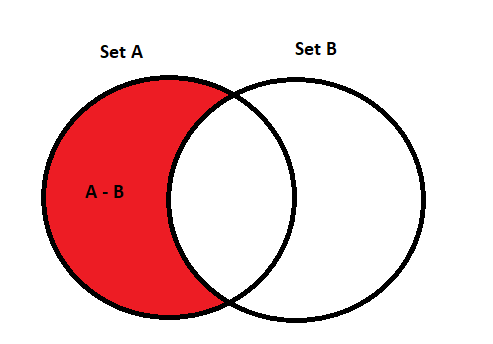
\includegraphics[width=.9\linewidth]{Set_Theory/2022-12-06_09-56-18_Set-Difference.png}
\end{center}



The cardinality of the difference is \(|A \setminus B|\) or \(|A| - |A \cap B|\). The reason why we have to subtract the cardinality of the intersection is because the intersection is counted twice. Once in \(A\) and once in \(B\).

An example of this is the difference of \(\{1,2\}\) and \(\{2,3\}\) is \(\{1\}\). The reason why this is the difference is because \(1 \in A\) and \(1 \notin B\). So \(1\) is in the difference.

\subsection{Complement}
\label{sec:org0891bd1}
The complement of a set is the set of all elements that are not in the set. We denote this as \(A^c\). A more rigorous definition of this is as follows:

\[
A^c \equiv \{x \mid x \notin A\}
\]

In terms of the universal set, the complement of a set is the set of all elements that are not in the set and are in the universal set. It is denoted as \(A^c = U \setminus A\). A more rigorous definition of this is as follows:

\[
A^c \equiv \{x \mid x \in U \land x \notin A\}
\]

\textbf{The cardinality of the complement is \(|U| - |A|\).} The reason why we have to subtract the cardinality of the set is because the set is counted twice. Once in \(U\) and once in \(A\).

An example of this is the complement of \(\{1,2\}\) is \(\{3,4\}\). The reason why this is the complement is because \(3 \in U\) and \(3 \notin A\). So \(3\) is in the complement. This of course depends on the universal set being \(\{1,2,3,4\}\).

\subsection{Logical Operations with Sets}
\label{sec:org1c76dc8}
We can relate sets to logical operations. The most common logical operations are conjunction, disjunction, and negation. We can relate these to sets as follows:

\begin{array}{l}
A \cup B \sim p \lor q \\
A \cap B \sim p \land q \\
\bar{A} \sim \neg p
\end{array}

The reason why we can do this is that the definition of a set, is based on a predicate. So we can relate the set to the predicate and the predicate to the logical operation. For example, the definition of a set is as follows:

\[
A \equiv \{x \mid x \in A\}
\]

So we can relate the set to the predicate as follows:

\[
A \equiv \{x \mid x \in A\} \equiv \{x \mid p(x)\}
\]

\section{Functions}
\label{sec:org9d5ce50}
A function, is the assignment of a single value \(b\in B\) to each element \(a\) in a set \(A\). We denote this as \(f: A \rightarrow B\). We can also call a function a mapping, transformation or a black box (in some cases even an oracle). A more rigorous definition of this is as follows:

\[
f: A \rightarrow B \equiv \{f(a) \mid a \in A\}
\]

We are mostly interested in what makes a function a function. So we will define what makes a function a function. A function is a function if the following conditions are met:
\begin{enumerate}
\item The domain of the function is a set
\item The range of the function is a set
\item The function is one-to-one
\item The function is onto
\end{enumerate}

A mathematical way to express this is as follows:

\[
\forall a \in A \exists ! b \in B \land f(a) = b
\]

The reasons why some assignments might not be functions is that not all elements in \(A\) are assigned to an element in \(B\). This is called a partial function. Another reason why some assignments might not be functions is that not all elements in \(B\) are assigned to an element in \(A\). This is called a surjection. Another reason why some assignments might not be functions is that not all elements in \(A\) are assigned to a unique element in \(B\). This is called a bijection.

How can we tell if a function is a function? We can tell if a function is a function by checking if the function is one-to-one and onto. If the function is one-to-one and onto, then the function is a function. If the function is not one-to-one and onto, then the function is not a function.

\subsection{Domain, Codomain \& Range}
\label{sec:org11ea42a}
If \(f(a) = b\), then we call \(a\) the \textbf{pre-image} and \(b\) the \textbf{image} of \(f\). We call \(A\) the \textbf{domain} of \(f\) and \(B\) the \textbf{codomain} of \(f\). We call \(f(A)\) the \textbf{range} of \(f\).

The main difference between the \textbf{codomain} and the \textbf{range} is that the \textbf{codomain} is the set of all possible images of \(f\) and the \textbf{range} is the set of all images of \(f\).


\subsection{One-to-One}
\label{sec:org6b165bf}
A function is one-to-one if each element in the range is assigned to a unique element in the domain. We denote this as \(f: A \rightarrow B\) is one-to-one. A more rigorous definition of this is as follows:

\[
f: A \rightarrow B \text{ is one-to-one } \equiv \forall a_1, a_2 \in A \land f(a_1) = f(a_2) \implies a_1 = a_2
\]

or simply: \(f(a_1) = f(a_2) \implies a_1 = a_2\).

If we want to check if a functions is one-to-one, we have to test if \(f(a_1) = f(a_2) \implies a_1 = a_2\) for all \(a_1, a_2 \in A\). If this is true for all \(a_1, a_2 \in A\), then the function is one-to-one.


\subsection{Onto}
\label{sec:orgb70e140}
A function is onto if each element in the codomain is assigned to an element in the domain. We denote this as \(f: A \rightarrow B\) is onto. This is to say that for each element in the codomain, there is an element in the domain that maps to it. A more rigorous definition of this is as follows:

\[
f: A \rightarrow B \text{ is onto } \equiv \forall b \in B \exists a \in A \land f(a) = b
\]

or simply: \(\forall b \in B \exists a \in A \land f(a) = b\).

To see if a function is onto, we have to test if \(\forall b \in B \exists a \in A \land f(a) = b\). If this is true for all \(b \in B\), then the function is onto. For example if \(f: \{1,2\} \rightarrow \{1,2,3\}\), then \(f(1) = 1\), \(f(2) = 2\) and \(f(3) = 3\). So \(f\) is onto. If \(f: \{1,2\} \rightarrow \{1,2\}\), then \(f(1) = 1\), \(f(2) = 2\) and \(f(3) = 3\). So \(f\) is not onto. In this case, the function is not onto because \(3\) is not assigned to an element in the domain.

\subsection{Composite Functions}
\label{sec:org1c1e13f}
We can combine functions to create composite functions. We can combine functions by applying one function to the output of another function. We denote this as \(f \circ g\). We can also call this function composition. A more rigorous definition of this is as follows:

\[
f \circ g \equiv \{f(g(a)) \mid a \in A\}
\]

If the \textbf{codomain} of \(g\) is the \textbf{domain} of \(f\), then we can combine \(g\) and \(f\) to create a composite function. We denote this as \(f \circ g: A \rightarrow C\).

When it comes to functions properties after composition we have the following properties:
\begin{enumerate}
\item \(f \circ g\) is one-to-one if \(f\) is one-to-one and \(g\) is one-to-one
\item \(f \circ g\) is onto if \(f\) is onto and \(g\) is onto
\end{enumerate}

If some of the functions are not one-to-one or onto, then the composite function is not one-to-one or onto.


\subsection{Inverse Functions}
\label{sec:org30ed0cf}
An inverse function is a function that undoes the effects of another function. We denote this as \(f^{-1}\). The definition is as follows:

\[
f^{-1} \equiv \{a \mid f(a) = b\}
\]

If \(f\) is one-to-one and onto, then \(f^{-1}\) is also one-to-one and onto.

\subsection{Partial Functions}
\label{sec:org646e3cf}
A partial function is a function that is not one-to-one or onto. We denote this as \(f: A \rightarrow B\) is a partial function. Definition:

\[
f: A \rightarrow B \text{ is a partial function } \equiv \exists a_1, a_2 \in A \land f(a_1) = f(a_2) \land a_1 \neq a_2
\]

or simply: \(\exists a_1, a_2 \in A \land f(a_1) = f(a_2) \land a_1 \neq a_2\). If this is true for some \(a_1, a_2 \in A\), then \(f\) is a partial function.

\subsection{Practice Questions}
\label{sec:orgc59fe15}
\begin{enumerate}
\item Let \(f: \mathbb{R} \rightarrow \mathbb{R}\) be defined by \(f(x) = x^2\). Is \(f\) one-to-one? Is \(f\) onto? Is \(f\) a partial function?
\begin{description}
\item[{Solution}] \(f\) is one-to-one because \(f(x) = f(y) \implies x = y\). \(f\) is not onto because \(f(x) = x^2\) and \(x^2\) is not in the domain. \(f\) is not a partial function because \(f(x) = f(y) \implies x = y\).
\end{description}
\item Let \(f: \mathbb{R} \rightarrow \mathbb{R}\) be defined by \(f(x) = x^2\). Is \(f^{-1}\) one-to-one? Is \(f^{-1}\) onto? Is \(f^{-1}\) a partial function?
\begin{description}
\item[{Solution}] \(f^{-1}\) is one-to-one because \(f^{-1}(x) = f^{-1}(y) \implies x = y\). \(f^{-1}\) is onto because \(f^{-1}(x) = x^2\) and \(x^2\) is in the domain. \(f^{-1}\) is not a partial function because \(f^{-1}(x) = f^{-1}(y) \implies x = y\).
\end{description}
\item Let \(f: \mathbb{R} \rightarrow \mathbb{R}\) be defined by \(f(x) = x^2\). Is \(f \circ f\) one-to-one? Is \(f \circ f\) onto? Is \(f \circ f\) a partial function?
\begin{description}
\item[{Solution}] \(f \circ f\) is one-to-one because \(f\) is one-to-one and \(f\) is one-to-one. \(f \circ f\) is onto because \(f\) is onto and \(f\) is onto. \(f \circ f\) is not a partial function because \(f \circ f\) is one-to-one and \(f \circ f\) is onto.
\end{description}
\item Let \(f: \mathbb{R} \rightarrow \mathbb{R}\) be defined by \(f(x) = x^2\). Is \(f \circ f^{-1}\) one-to-one? Is \(f \circ f^{-1}\) onto? Is \(f \circ f^{-1}\) a partial function?
\begin{description}
\item[{Solution}] \(f \circ f^{-1}\) is one-to-one because \(f\) is one-to-one and \(f^{-1}\) is one-to-one. \(f \circ f^{-1}\) is onto because \(f\) is onto and \(f^{-1}\) is onto. \(f \circ f^{-1}\) is not a partial function because \(f \circ f^{-1}\) is one-to-one and \(f \circ f^{-1}\) is onto.
\end{description}
\end{enumerate}

\section{Sequences}
\label{sec:orgd4ef528}

A sequence is a set of elements, which can be continued by using intuition or mathematical patterns. We denote this as \(\{a_n \mid n \in \mathbb{N}\}\). We will mostly focus on \textbf{arithmetic} sequences and \textbf{geometric} sequences.

\subsection{Arithmetic Sequences}
\label{sec:orge44db40}
An arithmetic sequence is a sequence where the difference between two consecutive terms is constant. We denote this as \(\{a_n \mid n \in \mathbb{N}\}\) where \(a_n = a_1 + (n-1)d\) for some \(a_1, d \in \mathbb{R}\). We can also write this as \(a_n = a_1 + nd\), where \(n\) is the \textbf{nth} term of the sequence and \(d\) is the \textbf{common difference}.

An arithmetic sequence is defined by the following properties:
\begin{enumerate}
\item \(a_n = a_1 + (n-1)d\)
\item \(a_n = a_1 + nd\)
\end{enumerate}

This sequence can also be thought of as a linear function. We can write this as \(a_n = f(n)\) where \(f(n) = a_1 + (n-1)d\). The main elements of a sequence are the \textbf{first term} and the \textbf{common difference}.

The expansion for the arithmetic sequence is as follows:

\begin{align}
a_1 = a_1 + 0d &= a_1 \\
a_2 = a_1 + 1d &= a_1 + d \\
a_3 = a_1 + 2d &= a_1 + 2d \\
a_4 = a_1 + 3d &= a_1 + 3d \\
\vdots &= \vdots \\
a_n = a_1 + (n-1)d &= a_1 + (n-1)d
\end{align}

\subsection{Geometric Sequences}
\label{sec:orgcab0ed1}
A geometric sequence is a sequence where the ratio between two consecutive terms is constant. We denote this as \(\{a_n \mid n \in \mathbb{N}\}\) where \(a_n = a_1 r^{n-1}\) for some \(a_1, r \in \mathbb{R}\). We can also write this as \(a_n = a_1 r^n\), where \(n\) is the \textbf{nth} term of the sequence and \(r\) is the \textbf{common ratio}.

An expansion of such as sequence can look something like this:

\begin{align}
a_1 &= a_1 \\
a_2 &= a_1 r \\
a_3 &= a_1 r^2 \\
a_4 &= a_1 r^3 \\
\vdots &= \vdots \\
a_n &= a_1 r^{n-1}
\end{align}

\subsection{Recurrence Relations}
\label{sec:org1bd5f43}
A recurrence relation is a sequence that is defined by a formula. We denote this as \(\{a_n \mid n \in \mathbb{N}\}\) where \(a_n = f(a_{n-1})\) for some \(f: \mathbb{R} \rightarrow \mathbb{R}\). It takes the previous term and applies a function to it to get the next term.

We can be told to find the closed formula for a sequence. This is a formula that can be used to find the nth term of a sequence.To do this, we need to use iteration and induction. We can use the following rules to find the closed formula for a sequence:
\begin{enumerate}
\item \(a_n = a_1 + (n-1)d\) where \(a_1, d \in \mathbb{R}\)
\item \(a_n = a_1 r^{n-1}\) where \(a_1, r \in \mathbb{R}\)
\item \(a_n = f(a_{n-1})\) where \(f: \mathbb{R} \rightarrow \mathbb{R}\)
\item \(a_n = f(a_{n-1}, a_{n-2})\) where \(f: \mathbb{R} \times \mathbb{R} \rightarrow \mathbb{R}\)
\end{enumerate}

In short, we need to find the pattern in the sequence and use that to find the closed formula.

\section{Summations}
\label{sec:org835f74b}
A summation is a way to add up a sequence of numbers. We denote this as \(\sum_{i=1}^n a_i\). There are many ways to define a summation. To find the sum of a sequence, we can use the following rules:
\begin{enumerate}
\item \(\sum_{i=1}^n i = \frac{n(n+1)}{2}\)
\item \(\sum_{i=1}^n i^2 = \frac{n(n+1)(2n+1)}{6}\)
\item \(\sum_{i=1}^n i^3 = \frac{n^2(n+1)^2}{4}\)
\item \(\sum_{i=1}^n C * f(i) = \frac{C}{1-r}\)
\end{enumerate}

If we subtract 1 from the upper bound, we can find the sum of the sequence. For example, \(\sum_{i=1}^n i = \sum_{i=0}^{n-1} i + n = \sum_{i=0}^{n-1} i + \sum_{i=n}^n i = \sum_{i=0}^{n-1} i + n = \frac{n(n-1)}{2} + n = \frac{n(n+1)}{2}\).

If we have nested summations, we can expand the far-right summation and include it in each iteration of the left summation.

\section{Divisibility}
\label{sec:org7f1f72e}
A number is divisible by another number if the remainder is 0. We denote this as \(a \mid b\) where \(a\) is the divisor and \(b\) is the dividend. We can also write this as \(a = q \cdot d + r\) where \(r\) is the remainder and \(q\) is the quotient. It is important to note that \(r\) is always less than \(d\) and always positive.

The elements in the primary equation are as follows:
\begin{enumerate}
\item \(a\) is the dividend
\item \(d\) is the divisor
\item \(q\) is the quotient
\item \(r\) is the remainder
\end{enumerate}

From this equation we gain two new operations, the \textbf{division} operation and the \textbf{modulus} operation. We can use these operations to find the remainder and quotient of a division problem.

If we perform division of a negative number, we cannot have a negative remainder. To solve this, we can add the divisor to the dividend until the remainder is positive. This is called the \textbf{floor division} operation. In other words, we want to 'overshoot' with the dividend and then compensate with the remainder.

\begin{itemize}
\item Division Function: This function is onto but not one-to-one
\item Modulus Function: This function neither one-to-one or onto
\end{itemize}


\subsection{Divisibility Rules}
\label{sec:org27645b5}
We can use divisibility rules to determine if a number is divisible by another number. The rules are as follows:
\begin{enumerate}
\item If \(a\) divides both \(b\) and \(c\), then \(a\) divides \(b+c\). Expression: \(a \mid b \land a \mid c \Rightarrow a \mid (b+c)\)
\item If \(a\) divides \(b\), then \(a\) divides any multiple of \(b\). Expression: \(a \mid b \implies a \mid bm\) for some \(m \in \mathbb{N}\)
\item If \(a\) divides \(b\) and \(b\) divides \(c\), then \(a\) divides \(c\). Expression: \(a \mid b \land b \mid c \Rightarrow a \mid c\)
\end{enumerate}

\section{Modular Arithmetic}
\label{sec:org70ad30f}
Modular arithmetic uses the modulus operation to find the remainder of a division problem. We use the notation \(a \equiv b \pmod{m}\) to denote that \(a\) is congruent to \(b\) modulo \(m\).

If we want to identify if two integers are congruent modulo \(m\), we can test this in the following way:
\begin{enumerate}
\item \(a \equiv b \pmod{m} \land b \equiv c \pmod{m} \Rightarrow a \equiv c \pmod{m}\)
\end{enumerate}

\textbf{In other words, if the remainder of the modulus operation is the same, then the two numbers are congruent modulo \(m\).}

\subsection{Rules of Modular Arithmetic}
\label{sec:org4d63c27}
We can use the following rules to perform modular arithmetic:
\begin{enumerate}
\item \(a \equiv b \pmod{m} \land c \equiv d \pmod{m} \Rightarrow a+c \equiv b+d \pmod{m}\)
\item \(a \equiv b \pmod{m} \land c \equiv d \pmod{m} \Rightarrow ac \equiv bd \pmod{m}\)
\item \(a \equiv b \pmod{m} \land c \equiv d \pmod{m} \Rightarrow a-c \equiv b-d \pmod{m}\)
\item \(a \equiv b \pmod{m} \land c \equiv d \pmod{m} \Rightarrow a/c \equiv b/d \pmod{m}\)
\item \(a \equiv b \pmod{m} \land c \equiv d \pmod{m} \Rightarrow a^c \equiv b^d \pmod{m}\)
\end{enumerate}

The difference between congruency and the modulo operation is that congruency is a relation between two numbers, while the modulo operation is an operation that returns a number. For example, \(a \equiv b \pmod{m}\) is a relation between \(a\) and \(b\), while \(a \pmod{m}\) is an operation that returns a number.

\subsection{Inverse of a Modulo}
\label{sec:orge827119}
We can find the inverse of a modulo by using the following equation: \(a \cdot a^{-1} \equiv 1 \pmod{m}\). In other words, if we multiply the inverse of a modulo by the modulo, we get 1 modulo \(m\).

To find the inverse of a modulo, we can use the Extended Euclidean Algorithm. This algorithm is as follows:
\begin{enumerate}
\item Set \(a = m \cdot q + r\) where \(q\) is the quotient and \(r\) is the remainder
\item Set \(b = a \cdot q + r\) where \(q\) is the quotient and \(r\) is the remainder
\item Repeat step 2 until \(r = 0\)
\item The inverse of \(m\) modulo \(a\) is \(q\) where \(q\) is the quotient of the last step
\end{enumerate}

For example, if we want to find the inverse of 3 modulo 7, we can use the Extended Euclidean Algorithm as follows:
\begin{enumerate}
\item \(7 = 3 \cdot 2 + 1\)
\item \(3 = 1 \cdot 3 + 0\)
\item \(r = 0\) so we stop
\item The inverse of 3 modulo 7 is 3
\end{enumerate}

\subsection{Practice Problems}
\label{sec:org0c04fd7}
\begin{enumerate}
\item \(2 \equiv 3 \pmod{5}\)

Solution: False, 2 is not congruent to 3 modulo 5

\item \(3 \equiv 4 \pmod{5}\)

Solution: False, 3 is not congruent to 4 modulo 5

\item \(4x \equiv 7 \pmod{5}\)

Solution: This is true when \(x = 0.5\) because \(4(0.5) \equiv 7 \pmod{5}\) is true.

\item \(x \equiv 3 \pmod{5} \land x \equiv 4 \pmod{5}\)

Solution: This is not true because \(3 \not\equiv 4 \pmod{5}\) so \(x \not\equiv 3 \pmod{5} \land x \not\equiv 4 \pmod{5}\)
\end{enumerate}

Practice problems using powers of modular arithmetic:

\begin{enumerate}
\item \(2^3 \equiv 8 \pmod{5}\)

Solution: This is true because \(2^3 = 8 \equiv 8 \pmod{5}\)
\end{enumerate}



\section{Integer Representation}
\label{sec:org2b04a3f}
Integers can be represented in many ways. In every day life, we use the base 10 system. This means that we use the digits 0-9 to represent numbers. We can also use the base 2 system. This means that we use the digits 0-1 to represent numbers. We can also use the base 16 system. This means that we use the digits 0-9 and A-F to represent numbers. We can also use the base 26 system. This means that we use the digits A-Z to represent numbers.

If we want to convert the value of base \(b\) to base \(b'\), we can use the following formula:

\[
n = a_k b^k + a_{k-1} b^{k-1} + \cdots + a_1 b + a_0
\]

The general algorithm for calculating the number representation is as follows:
\begin{enumerate}
\item Divide the number by the base
\item Take the remainder and add it to the list of digits
\item Repeat until the number is 0
\end{enumerate}

In mathematics:

\begin{align}
n = a_0 + bq_0 \\
n = a_1 + b(a_1 + bq_1) \\
n = a_2 + b(a_1 + b(a_2 + bq_2))
\end{align}

\section{Binary Representation}
\label{sec:org9740234}
Binary representation is the representation of numbers in base 2. We can use the following rules to convert from base 10 to base 2:
\begin{enumerate}
\item Divide the number by 2
\item Take the remainder and add it to the list of digits
\item Repeat until the number is 0
\end{enumerate}

To then put together the binary string we take each bit in reverse order and put it together. For example, the binary representation of 13 is 1101.

To make life a bit easier, we can use a table to convert from base 10 to base 2. The table is made up of the powers of 2 and the digits 0-1.
\begin{center}
\begin{tabular}{rrrrrrrr}
2\textsuperscript{7} & 2\textsuperscript{6} & 2\textsuperscript{5} & 2\textsuperscript{4} & 2\textsuperscript{3} & 2\textsuperscript{2} & 2\textsuperscript{1} & 2\textsuperscript{0}\\
\hline
128 & 64 & 32 & 16 & 8 & 4 & 2 & 1\\
\end{tabular}
\end{center}

\section{Hexadecimal Representation}
\label{sec:orgf905e86}
Hexadecimal representation is the representation of numbers in base 16. We can use the following rules to convert from base 10 to base 16:
\begin{enumerate}
\item Divide the number by 16
\item Take the remainder and add it to the list of digits
\item Repeat until the number is 0
\end{enumerate}

To then put together the hexadecimal string we take each digit in reverse order and put it together. For example, the hexadecimal representation of 15816 is 3DC8. The steps taken to get to this number are as follows:
\begin{enumerate}
\item 15816 / 16 = 988 remainder 8
\item 988 / 16 = 61 remainder 12 (12 is C in hexadecimal)
\item 61 / 16 = 3 remainder 13 (13 is represented as D in hexadecimal)
\item 3 / 16 = 0 remainder 3
\item 3DC8
\end{enumerate}

\section{Prime Numbers}
\label{sec:org1cf4f80}
A prime number is a number that is only divisible by 1 and itself. We can use the following rules to determine if a number is prime:
\begin{enumerate}
\item If \(n\) is divisible by \(a\), then \(n\) is not prime
\item If \(n\) is not divisible by \(a\), then \(n\) is prime
\end{enumerate}

Any number that is not prime is called a composite number. This relates to the Fundamental Theorem of Arithmetic. This theorem states that every integer greater than 1 can be expressed as a product of prime numbers. This theorem is important because it allows us to factorize numbers.

How to determine if a number is a prime or composite? We can use the following proposition:

\[
(n \text{ is composite})  \Leftrightarrow \exists a \in \mathbb{N} (( a \mid n) \land (a \neq 1) \land (a \neq n))
\]


\section{Algorithms}
\label{sec:org6185414}
An algorithm is a collection of instructions that are made to solve a problem. To create any algorithm, we need three basic components:
\begin{description}
\item[{Sequence}] A sequence is a list of instructions that are executed in order
\item[{Selection}] A selection is a list of instructions that are executed based on a condition
\item[{Iteration}] An iteration is a list of instructions that are executed multiple times
\end{description}

\subsection{Complexity of Algorithms}
\label{sec:org4c29887}
The complexity of an algorithm is given by the relation between the input size and the number of steps required to solve the problem. We can use the following notations to describe the complexity of an algorithm:
\begin{description}
\item[{\(O(n)\)}] This notation describes the worst case scenario for an algorithm. This means that the algorithm will take at least this amount of time to solve the problem.
\item[{\(\Omega(n)\)}] This notation describes the best case scenario for an algorithm. This means that the algorithm will take at most this amount of time to solve the problem.
\item[{\(\Theta(n)\)}] This notation describes the average case scenario for an algorithm. This means that the algorithm will take this amount of time to solve the problem.
\end{description}

We will not need omega and theta notation for the exam, but it is good to know.
\subsection{Big O Notation}
\label{sec:org7f55609}
Big O notation is used to describe the worst case scenario for an algorithm. We can use the following rules to determine the complexity of an algorithm:

The idea of this notation is that we can use it to compare the complexity of different algorithms. For example, if we have two algorithms that solve the same problem, we can use big O notation to determine which algorithm is better. If one algorithm is \(O(n)\) and the other is \(O(n^2)\), then the first algorithm is better than the second algorithm.

\begin{center}
\begin{tabular}{lll}
Algorithm & Complexity & Example\\
\hline
\(O(1)\) & Constant & Finding the first element in a list\\
\(O(\log n)\) & Logarithmic & Binary search\\
\(O(n)\) & Linear & Finding the maximum value in a list\\
\(O(n \log n)\) & Linearithmic & Merge sort\\
\(O(n^2)\) & Quadratic & Bubble sort\\
\(O(n^3)\) & Cubic & Matrix multiplication\\
\(O(2^n)\) & Exponential & Tower of Hanoi\\
\(O(n!)\) & Factorial & Travelling salesman problem\\
\end{tabular}
\end{center}

Contrary to intuition, to solve a large problem you should always use the most efficient algorithm, but for a smaller size, higher complexity algorithms are better.

\section{Greatest Common Divisor}
\label{sec:orgf11c424}
The greatest common divisor of two numbers is the largest number that divides both numbers. We can easily find this if we know the factorizations of each number. Another way to find the greatest common divisor is to use Euclid's algorithm. This algorithm is as follows:
\begin{enumerate}
\item Let \(a\) be the larger number and \(b\) be the smaller number
\item Divide \(a\) by \(b\) and take the remainder
\item If the remainder is 0, then \(b\) is the greatest common divisor
\item If the remainder is not 0, then set \(a\) to \(b\) and \(b\) to the remainder
\item Repeat until the remainder is 0
\end{enumerate}

An example of this algorithm is as follows:
\begin{enumerate}
\item Let \(a = 24\) and \(b = 16\)
\item \(24 \div 16 = 1\) remainder \(8\)
\item \(16 \div 8 = 2\) remainder \(0\)
\item \(b = 8\) is the greatest common divisor
\end{enumerate}

\subsection{Least Common Multiple}
\label{sec:org89f0f1d}
The least common multiple of two numbers is the smallest number that is divisible by both numbers. We can easily find this if we know the factorizations of each number. Another way to find the least common multiple is to use the following formula:

\[
\text{lcm}(a, b) = \frac{a \cdot b}{\text{gcd}(a, b)}
\]

\section{Applications of Number Theory}
\label{sec:org3296a51}
Number theory is used in many different fields. Some of these fields are as follows: cryptography, coding theory, and combinatorics.

\subsection{Databases}
\label{sec:orgbfb9dd9}
If we know the number of records in a database and who much space they take up, swell as the starting position, we can use the following formula to determine the position of the nth record:

\[
\text{position} = \text{starting position} + \text{record size} \cdot (n - 1)
\]

\subsection{Hash Functions}
\label{sec:orge8e8007}
If we want to store some records into a database, we can use a hash function which will map each record to a unique location in the database. This is done by taking the record and applying a hash function to it. The hash function will then return a number which is the location of the record in the database. We might use the \(mod\) operator to create a hash function.

If each entry has some numerical value we can use \(mod 10\) to map it to a location in the database. This method is not very practical because we might get some sort of collision. A collision is when two records map to the same location in the database. To avoid collisions we can make use of a secondary hash function.

\subsection{Asymmetric Encryption}
\label{sec:org6e09c0c}
Asymmetric encryption is a method of encryption that uses two keys. One key is used to encrypt the message and the other key is used to decrypt the message. The two keys are called the \textbf{public key} and the \textbf{private key}. The public key is used to encrypt the message and the private key is used to decrypt the message. The public key is made public and the private key is kept secret.

\section{Relations}
\label{sec:org4a2b4ee}
A relation is a set of ordered pairs. It is also a subset of the Cartesian product of the set. We can use the following notation to represent a relation:

\[
R = \{(x, y) \mid x \in A \land y \in B\}
\]

The easiest way to represent a relation is to use a table. The table will have the elements of the first set as the rows and the elements of the second set as the columns. If the ordered pair \((x, y)\) is in the relation, then we will put a \(1\) in the cell that corresponds to the row \(x\) and the column \(y\). If the ordered pair \((x, y)\) is not in the relation, then we will put a \(0\) in the cell that corresponds to the row \(x\) and the column \(y\).

Here is an example of a relation:

\[
R = \{(1, 2), (1, 3), (2, 1), (2, 3), (3, 1), (3, 2)\}
\]

We can represent this relation as a table as follows:

\begin{array}{c|ccc}
& 1 & 2 & 3 \\
\hline
1 & 0 & 1 & 1 \\
2 & 1 & 0 & 1 \\
3 & 1 & 1 & 0
\end{array}

The relationship between functions and relations is that a function is a relation where each ordered pair has a unique first element.

To find the cardinality of a relation for a \textbf{single set}, we can use the following formula:

\[
2^{n^2}
\]

This is because there are \(2\) possibilities for each ordered pair. The ordered pair can either be in the relation or it can not be in the relation. If we have \(n\) elements in the set, then there are \(n^2\) ordered pairs. Therefore, there are \(2^{n^2}\) possible relations.

This should also be equivalent to the power set of the Cartesian product of the set.


\subsection{Reflexive Relations}
\label{sec:org0185d96}
A relation is reflexive if it contains the ordered pair \((x, x)\) for every element \(x\) in the set. We can use the following notation to represent a reflexive relation:

\[
R = \{(x, y) \mid x \in A \land y \in A \land x = y\}
\]

As a matrix, it would look like this:

\begin{array}{c|ccc}
& 1 & 2 & 3 \\
\hline
1 & 1 & 0 & 0 \\
2 & 0 & 1 & 0 \\
3 & 0 & 0 & 1
\end{array}

\subsection{Symmetric Relations}
\label{sec:org5b0b110}
A relation is symmetric if it contains the ordered pair \((x, y)\) for every ordered pair \((y, x)\). We can use the following notation to represent a symmetric relation:

\[
R = \{(x, y) \mid x \in A \land y \in A \land (y, x) \in R\}
\]

As a matrix, it would look like this (or any other symmetric relation):

\begin{array}{c|ccc}
& 1 & 2 & 3 \\
\hline
1 & 0 & 1 & 1 \\
2 & 1 & 1 & 1 \\
3 & 1 & 1 & 0
\end{array}


\subsection{Antisymmetric Relations}
\label{sec:orgcb4bb64}
If a relation is antisymmetric, it will it will contain some order pair \((x,y)\) but not \((y,x)\) for every ordered pair \((x,y)\). We can use the following notation to represent an antisymmetric relation:

\[
R = \{(x, y) \mid x \in A \land y \in A \land (x, y) \in R \land (y, x) \notin R\}
\]

\subsection{Transitive Relations}
\label{sec:org82d5332}
A relation is transitive if it contains the ordered pair \((x, z)\) for every ordered pair \((x, y)\) and \((y, z)\). We can use the following notation to represent a transitive relation:

\[
R = \{(x, z) \mid x \in A \land z \in A \land (x, y) \in R \land (y, z) \in R\}
\]

What its saying is that the relation will be transitive if for every \(n\) steps, we can get from \(x\) to \(z\) in just one step.

\subsection{Composite Relations}
\label{sec:org664c4d2}
We can combine two relations to create a composite relation. The composite relation will contain the ordered pair \((x, z)\) if the first relation contains the ordered pair \((x, y)\) and the second relation contains the ordered pair \((y, z)\). We can use the following notation to represent a composite relation:

\[
R \circ S = \{(x, z) \mid x \in A \land z \in A \land (x, y) \in R \land (y, z) \in S\}
\]

We can us \textbf{powers of a binary relation} to represent the composite relation. The \$n\$th power of a binary relation will contain the ordered pair \((x, z)\) if the relation contains the ordered pair \((x, y)\) and the relation contains the ordered pair \((y, z)\) \(n\) times.

\section{Directed Graphs}
\label{sec:orge538cba}
If we want to represent a relation, we can use a directed graph. A directed graph is a graph where the edges have a direction. The edges can be represented by arrows. The arrows will point from the first element of the ordered pair to the second element of the ordered pair. If we have an ordered pair \((x, y)\) in the relation, then we will have an arrow from \(x\) to \(y\).

An example of a directed graph is the following:

\begin{center}
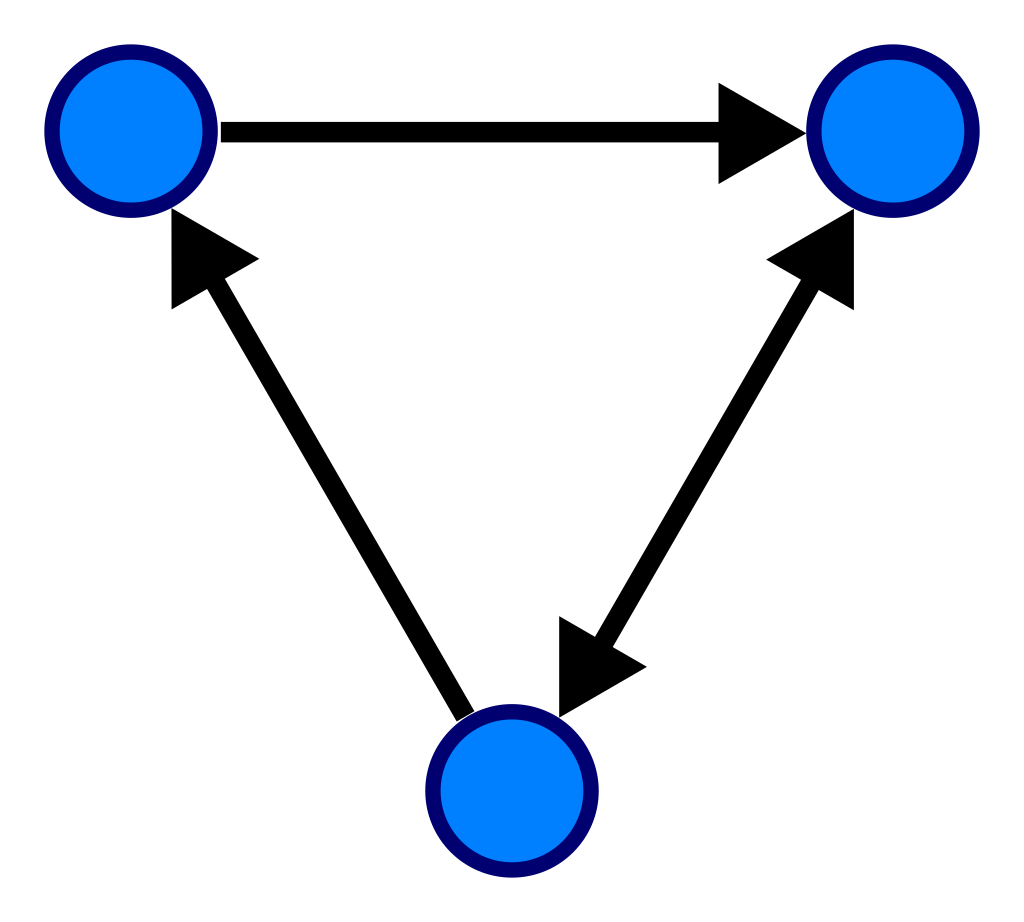
\includegraphics[width=.9\linewidth]{Directed_Graphs/2022-12-06_17-07-14_1024px-Directed.svg.png}
\end{center}

\section{Grammars}
\label{sec:org4b532d9}
A grammar is a set of rules that can be used to generate strings. The strings that are generated by the grammar are called the language of the grammar. The language of the grammar is the set of all strings that can be generated by the grammar. The language of the grammar is denoted by \(L(G)\).

\subsection{Railroad Diagrams}
\label{sec:orgf146329}


\begin{description}
\item[{Vocabulary}] This is a set of symbols which we use to represent the language of the grammar. The vocabulary of the grammar is denoted by \(V\).
\item[{Grammar}] This is a set of rules that can be used to generate strings. The grammar is denoted by \(G\). It is a combination of the vocabulary. By using grammar and vocabulary, we can generate strings which are part of \textbf{formal language}.
\end{description}


An example of a railroad diagram is the following:

\begin{center}
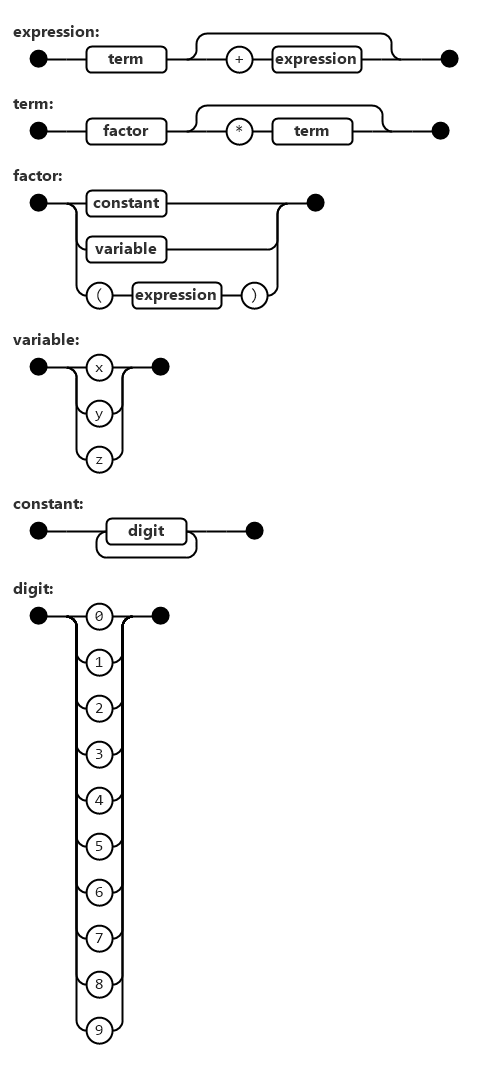
\includegraphics[width=.9\linewidth]{Grammars/2022-12-06_17-15-45_Syntax-diagram-example.png}
\end{center}

We write the railroad diagram as follows (not the one above):

\begin{verbatim}
<expression> ::= <term> | <term> "+" <expression>
<term>       ::= <factor> | <factor> "*" <term>
<factor>     ::= <constant> | <variable> | "(" <expression> ")"
<variable>   ::= "x" | "y" | "z"
<constant>   ::= <digit> | <digit> <constant>
<digit>      ::= "0" | "1" | "2" | "3" | "4" | "5" | "6" | "7" | "8" | "9"
\end{verbatim}


\emph{more coming soon}
\end{document}